\begin{frame}{Permissions}
  \begin{columns}
    \column{5.5cm}
    \footnotesize

    \textbf{Android}\\
    Einstellungen -> Apps -> Appname -> Berechtigungen ändern\\
    \vspace{0.2cm}
    Einstellungen -> Apps -> Zahnrad -> Appberechtigungen\\
    \vspace{0.5cm}

    \textbf{iOS}\\
    Einstellungen -> Privatsphäre -> Berechtigungsname\\
    \vspace{0.5cm}

    In den neuesten Versionen: Entscheidung bei erster Benutzung

    \column{5cm}

    \begin{center}
      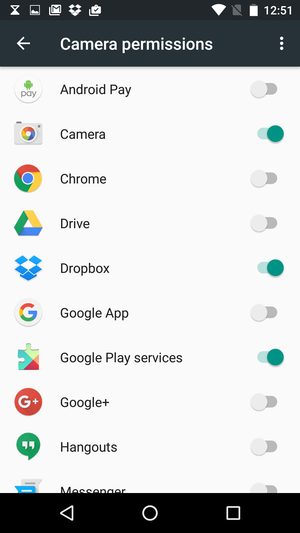
\includegraphics[width=3.5cm]{img/permissions-android.png}
    \par\end{center}
  \end{columns}
\end{frame}

\note{Die Berechtigungen bzw. Permissions auf mobilen Geräten informieren darüber welche Daten die App sehen kann. Vorsicht ist unter anderem bei Identität, Standort, Kontaktliste und Dateizugriff (Bilder/Videos etc.) geboten. Man sollte seinen Menschenverstand benutzen, um zu entscheiden, ob eine App die geforderten Berechtigungen wirklich benötigt und haben sollte. Bei neueren Versionen von Android und iOS kann man Apps detailliert Berechtigungen wegnehmen bzw. gar nicht erst erlauben.}
